  \documentclass[12pt]{article}

\usepackage{sbc-template}
\usepackage{float}
\usepackage{graphicx}
\usepackage{caption}
\usepackage{subcaption}
\usepackage[T1]{fontenc}
\usepackage[latin1]{inputenc}
\usepackage[brazil]{babel}

\let\oldemptyset\emptyset
\let\emptyset\varnothing

\sloppy
\captionsetup[figure]{labelsep=period}

\title{Recommendation of Yelp's Reviewers: Who Should You Listen to?}

\author{Luciana B. Maroun\inst{1}, Izabela K. T. Maffra\inst{1}}

\address{Universidade Federal de Minas Gerais (UFMG)
  \email{\{lubm,karennina\}@dcc.ufmg.br}
}

\begin{document} 

\maketitle

\renewcommand{\figurename}{Figure}
\renewcommand{\tablename}{Table}

\begin{abstract}
Online ratings are nowadays one of the most trusted sources of consumer
confidence when they need to decide which business to choose. As a matter of
fact, reviews have become so abundant that many times the task of deciding upon
whether or not to elect a business is getting increasingly difficult -- each
person has their own values and intrinsic characteristics that contribute to
forming an opinion. In this work, we discriminate relevant users from a review
website considering the perspective of a second user. This way, we are able to
infer what would be the individuals that think alike certain user and recommend
their reviews amongst a plethora of diverse opinions.
\end{abstract}

\section{Introduction}
Consumer reviews have revolutionized the way that people choose which businesses
to attend. It is now very common to turn to the web in order to make everyday
decisions, such as where to eat or where to get a haircut.
Yelp\footnote{www.yelp.com} is an opinion and experience sharing system about
businesses of several kinds. In this platform, a user is able to write their
impressions about certain place and rate it with a score from one to five stars.
Therefore, before choosing where to go, someone can investigate what others
think about different places and make a decision with a wider knowledge basis.

To illustrate the importance of such platforms, a survey recently discovered
that 64\% of all consumers scan reviews before choosing a service \cite{survey}.
Businesses' owners, on the other hand, are being forced to direct their
attention to such platforms, since it was found that an extra half star on
average rating increase sales on 19\% \cite{study}.

However, users differ in values and taste. Thus, an opinion might be useful for
someone and not so much for somebody else. Knowing the profile of an individual
is helpful to understand the viewpoint behind a review and decide if its
adequate considering the reader's angle.

The purpose of this work is to identify important reviewers on Yelp for
determined user in order to recommend reviews aligned with the readers'
preferences and style. Different features might be helpful in this process,
including the friendship network of reviewers. In this work, we analyze the
relevance of the friendship network in users profiling as well as of a hidden
friendship network --- defined by users who are similar but are not connected on
the social network. By encountering individuals with similar opinions, validated
by the homophilly on the network, we recommend the reviews of those to the
reader and reduce the burden of manually searching for relevant viewpoints.


\section{Dataset}
The data used consists of a set of reviews, business, users and related content
of Yelp's website regarding the metropolitan area of Phoenix released for a
challenge\footnote{www.yelp.com/dataset\_challenge}. There are $15,585$
businesses, $70,817$ users and $335,022$ reviews, which covers a period from
$2005-02-01$ until $2014-01-28$.

Yelp also contains an online social network (OSN), thus users are able to be
friends of each other. This network, however, is not the main purpose of the
platform and does not entirely represent the true interaction between
individuals --- sometimes the motivation of connection is not really a
friendship, but similar businesses preferences and reviewing behavior. A great
part of the users, however, does not even have any friends: only $30,255$ of
them are socially connected. This proves that this network is not enough for
discovering reference reviewers, demanding an extrapolation with unobserved
edges.


\section{Network Analysis}
As previously mentioned, the friendship network of Yelp is rather incomplete:
the majority of users does not have any connections. The users that participate
on the social network, however, are highly connected, since $40.92$\% of them
are in the large connected component, which means that only $1.80$\% of the OSN
participants are absent. The average degree of the whole network is $4.68$ and
the clustering coefficient is $0.06$. Figure~\ref{fig:plot} depicts a plot of the
network. In this plot, nodes who are friends tend to be closer than nodes who are
not friends. We can note a central core of users which are more highly connected, as well
as a cloud of disconnected users.

\begin{figure}[ht!]
\centering
\includegraphics[scale=0.5]{img/plot}
\caption{The visualization of the friendship network.}
\label{fig:plot}
\end{figure}

Yelp provides an option for users to vote in reviews that they found useful.
Figure~\ref{fig:clo_use} relates the closeness centrality to the total useful
votes received by a user. We observe that there are roughly three situations:
users with low centrality and low usefulness; users with high centrality and low
usefulness; and users with high centrality and high usefulness. There is not
such a configuration in which users with high usefulness have low centrality.
This is a motivation to consider the network structure as an evidence for
profile of reviewers.

\begin{figure}[H]
\centering
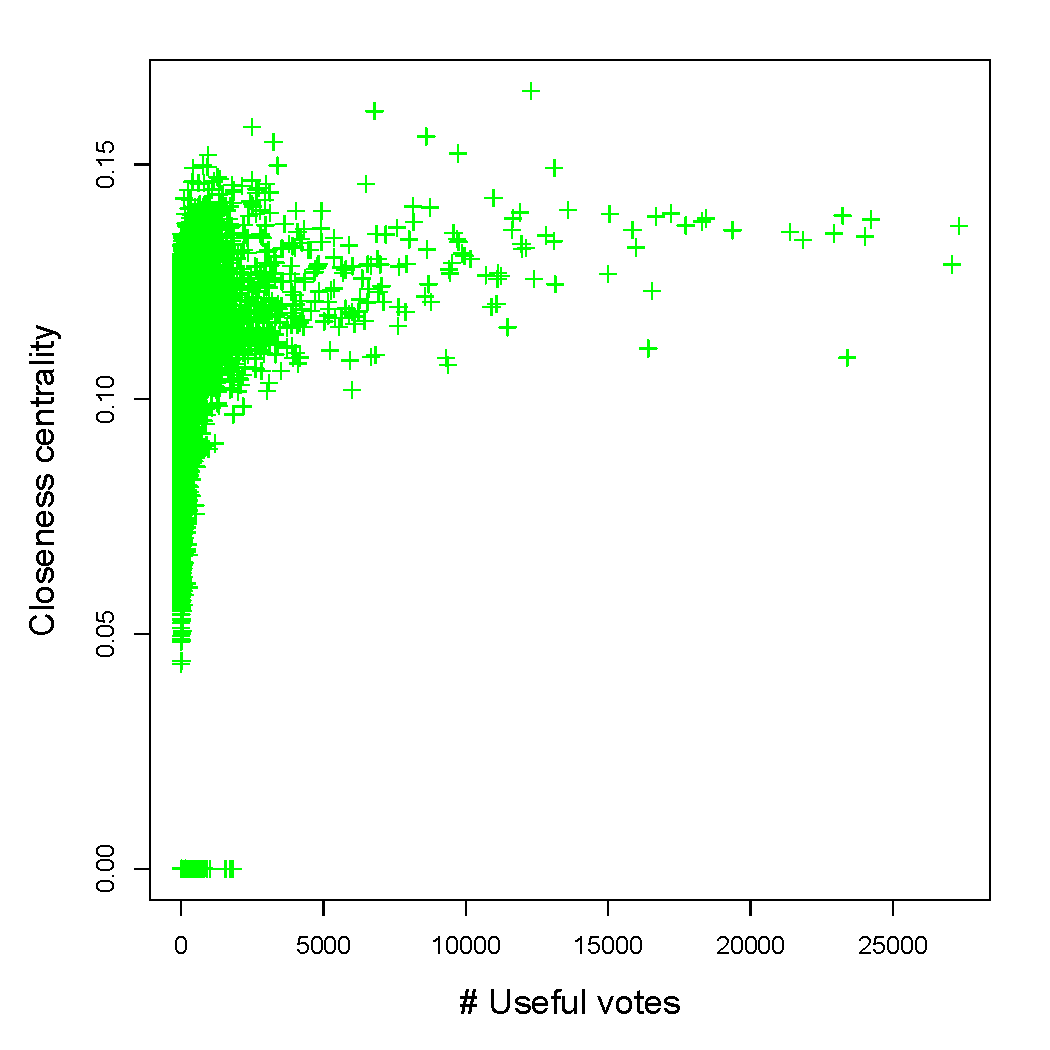
\includegraphics[scale=0.5]{img/close_useful_scatter}
\caption{Correlation between closeness centrality and the number of useful votes for a reviewer.}
\label{fig:clo_use}
\end{figure}

The third set of users cited, a minority, corresponds to reviewers that
influence a lot of people. However, few useful votes might indicate that those
reviewers provide important experiences for only certain kind of people. Thus,
it is necessary to investigate further those reviewers in order to present the
information they provide to the ones interested.

\subsection{Homophilly Investigation}

Aiming to validate the presence of homophilly in the network, it was conducted
the following experiment: for each edge on the network, the business overlap was
computed considering the jaccard similarity of reviewed establishments; a
similar process was perfomed for a modified graph with the same nodes and number
of edges, which were randomly assigned to pairs. The empirical cumulative
distribution of the overlap values are depicted on figure \ref{fig:bus_olap}. We
observe a clear difference between the real and the random graphs --- the second
practically do not contain positive overlaps, while the first present some.

\begin{figure}[H]
\centering
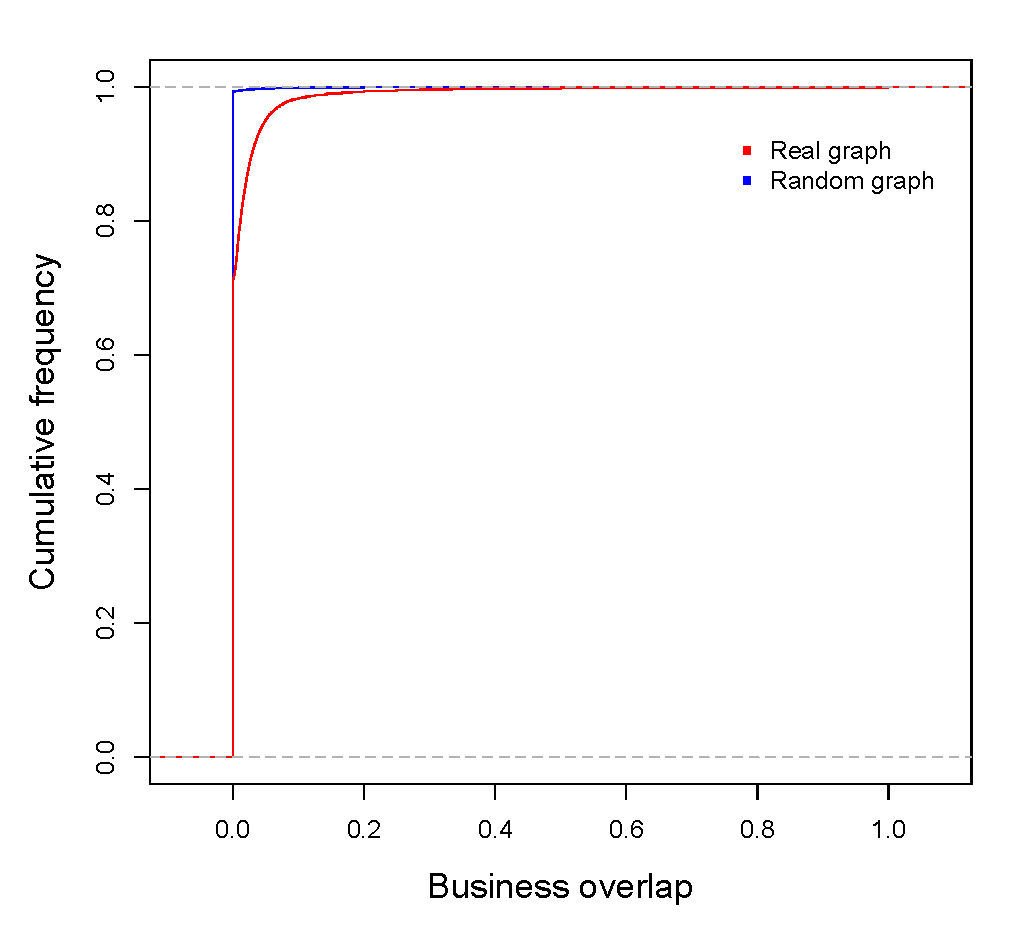
\includegraphics[scale=0.5]{img/ecdf_bus_olap}
\caption{Empirial cumulative distribution of business overlap on real and random graphs.}
\label{fig:bus_olap}
\end{figure}


\subsection{Temporal Effect}
Another important aspect when considering similarity of opinions is the date of
the review. People that visit a place in the same day are more likely to
experience the same events and to have approximate opinions. The figure
\ref{fig:rat_heat} contains the correlation reviews given to the same
establishment by friends in the same day \ref{fig:fri_eq}, not friends in the
same day \ref{fig:nfri_eq}, friends in different days \ref{fig:fri_dif} and not
friends in different days \ref{fig:nfri_dif}. The results are normalized ---
each cell represents the percentage of co-occurences for the given column. For
example, in figure \ref{fig:fri_eq}, if one individual rates $1$, there is a
proportion of $70$\% of their friends who rated $1$, nearly $30$\% who rated $2$
and practically $0$\% who rated $3$, $4$ or $5$.

\begin{figure}[H]
  \centering
  \begin{subfigure}[b]{0.5\textwidth}
    \captionsetup{font=small}
    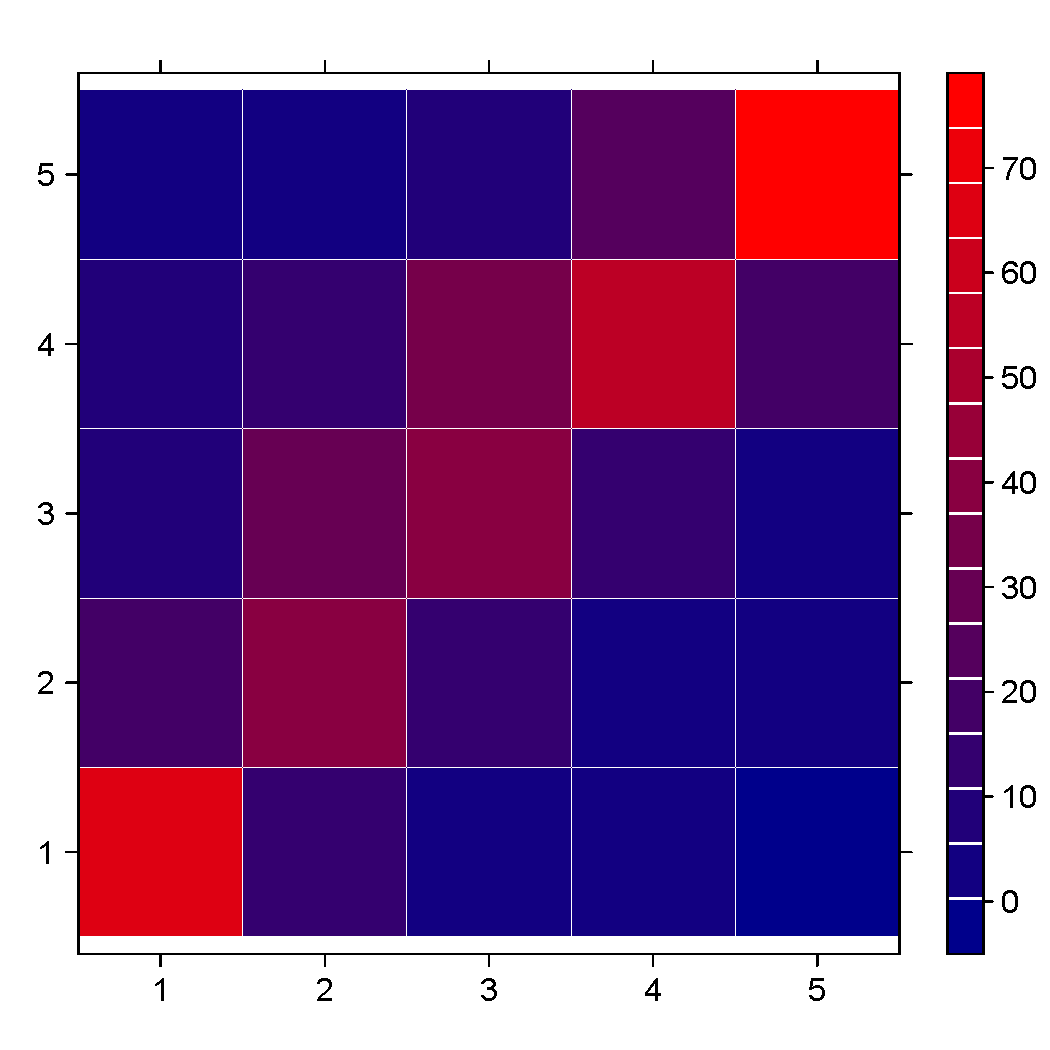
\includegraphics[width=\textwidth]{img/amig_eq_n}
    \caption{Friends in same day.}\label{fig:fri_eq}
  \end{subfigure}%
  ~
  \begin{subfigure}[b]{0.5\textwidth}
    \captionsetup{font=small}
    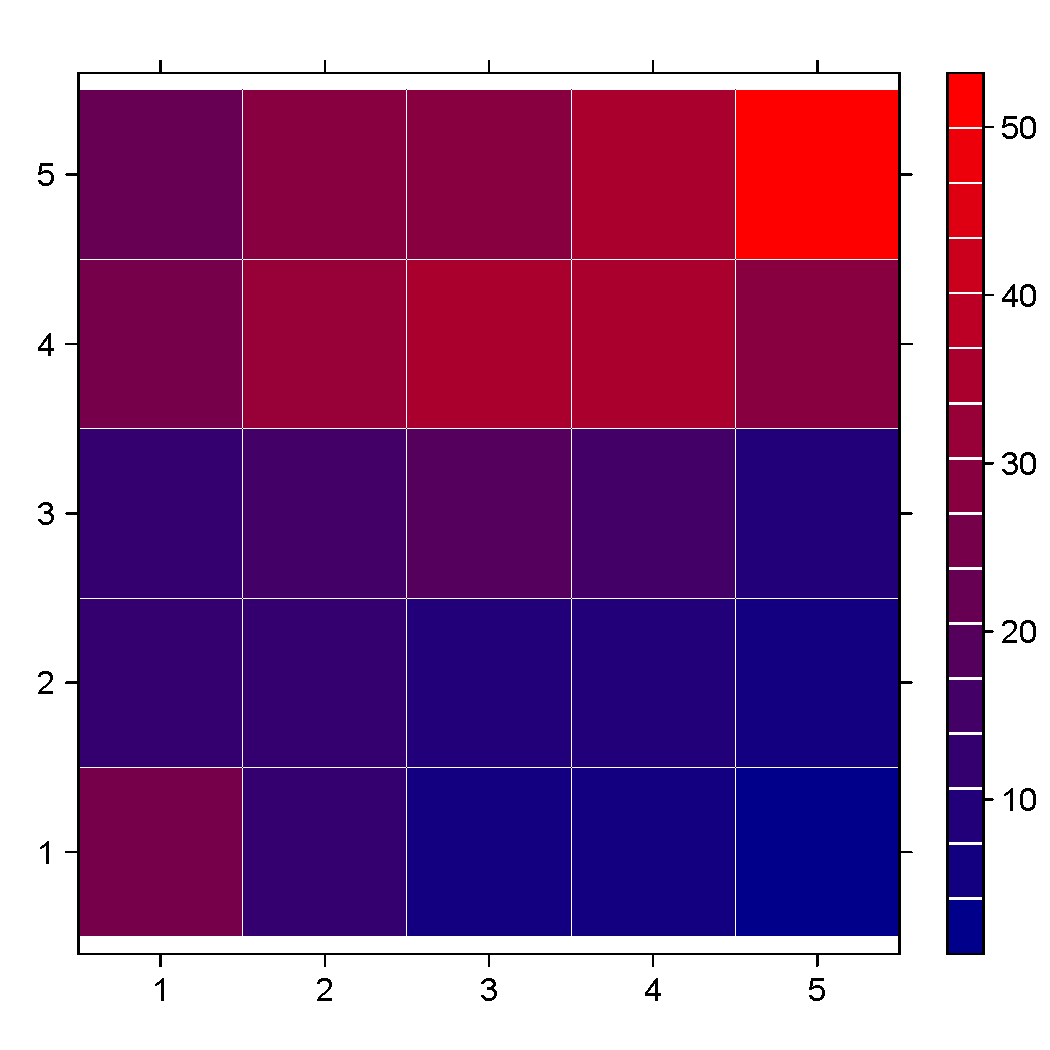
\includegraphics[width=\textwidth]{img/namig_eq_n}
    \caption{Not friends in same day.}\label{fig:nfri_eq}
  \end{subfigure}
  ~
  \begin{subfigure}[b]{0.5\textwidth}
    \captionsetup{font=small}
    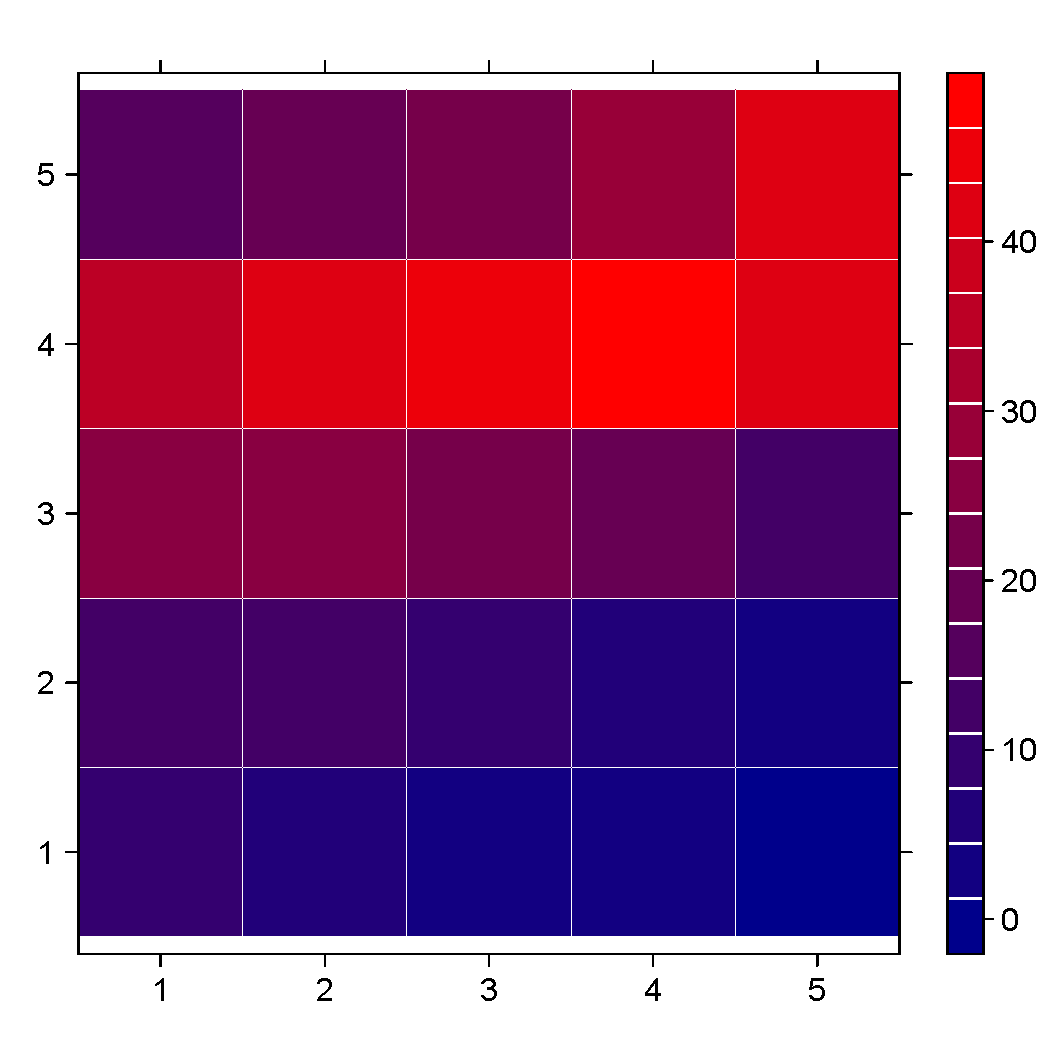
\includegraphics[width=\textwidth]{img/amig_dif_n}
    \caption{Friends in different days.}\label{fig:fri_dif}
  \end{subfigure}%
  ~
  \begin{subfigure}[b]{0.5\textwidth}
    \captionsetup{font=small}
    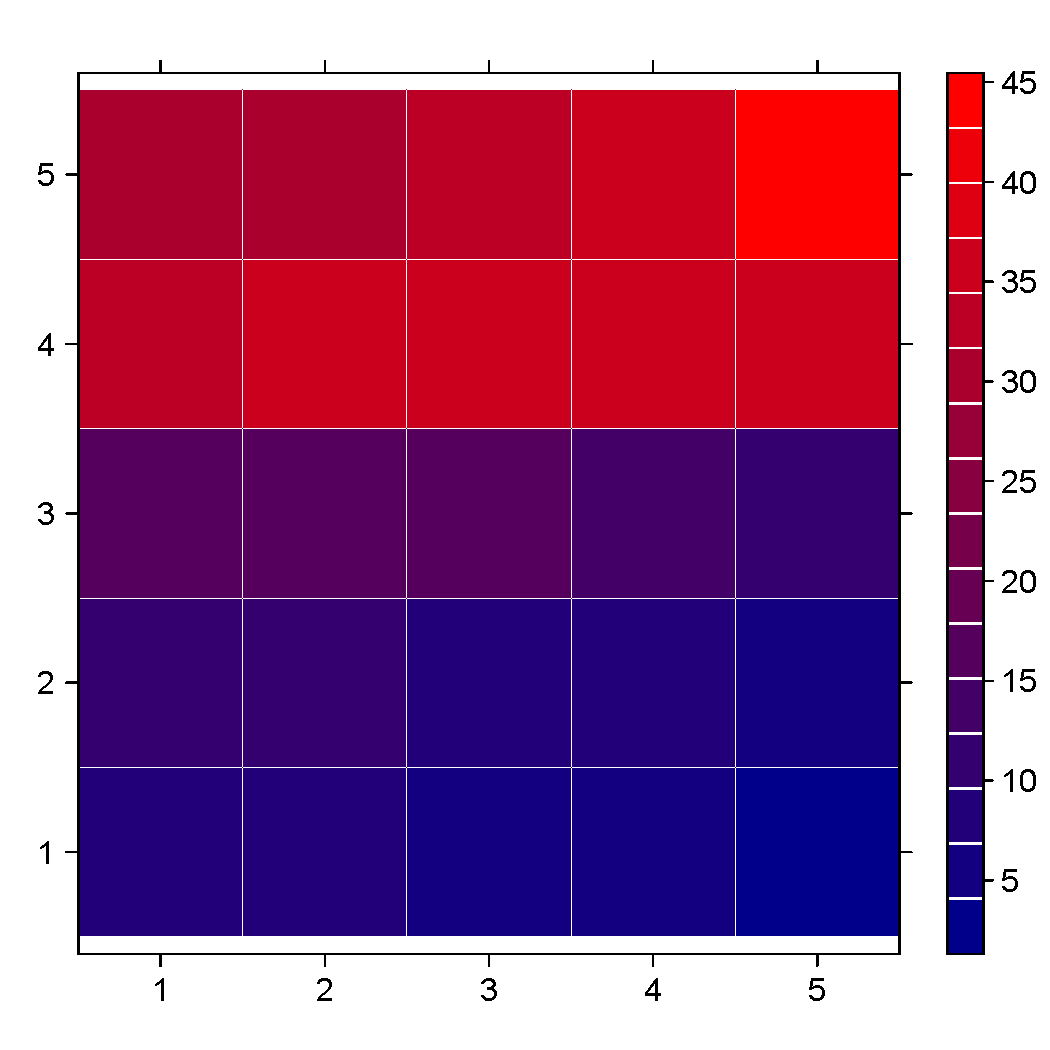
\includegraphics[width=\textwidth]{img/namig_dif_n}
    \caption{Not friends in different days.}\label{fig:nfri_dif}
  \end{subfigure}
  ~
  \caption{Correlation of votes between pair of users percentual by column.}
  \label{fig:rat_heat}
\end{figure}

We can observe a gradative pattern from a strong correlation of ratings to
almost no correlation, in which the proportion of votes on each value rules
the intensity.

An interesting observation is that there is much less agreement
between people who visited a place in the same day and are not friends. If we infer that
friends had the experience together, this is a very interesting fact: one might be affected by the
mood and the way a friend is feeling about a mutual experience.

The heatmaps are very alike for different days, so the friendship plays no special role here.

\subsection{Hidden Relationships}
RECAST\cite{vaz2013recast} is an algorithm that identifies relationships in
dataset of encounters of people and classifies the relationship between each
pair of individuals as friend, bridge, acquaintance or random. Applying the
method for reviews written in the same date, supposing that the day of
the review is the same of the attendance, we obtain the result presented on
table \ref{tab:recast}.

\begin{table}[H]
\begin{tabular}{l|rrrr}
Relationship & \# Friends & \# Bridges & \# Acquaintances & \# Random \\ 
\hline
Friends on Yelp & 69 & 21 & 689 & 634 \\
Not Friends on Yelp & 16 & 3 & 5876 & 13205 \\
\end{tabular}
\caption{Discovered relationships using RECAST.}
\label{tab:recast}
\end{table}

We can observe a great value for acquaintances for Yelp users which are not
friends. This indicates the potential of hidden relationships, which might be an
indication of some similarity of opinions.

\section{Recommendation of Reviewers}
Collaborative filtering is an algorithm which combines the evaluation of
users in a bunch of topics in order to predict users rating in unseen ones. In
this process, the evaluated elements have a set of attributes that define them
and are closely related to their scores. The users, on the other hand, have a
representative vector which are coefficients for the attributes and informs the
importance given for each one of them. 

Considering this model, it is possible to
discover people with similar interests, which does not necessarily have to be friends in Yelp,
by filtering those with small euclidian distance.

The algorithm basically solves an optmization problem which consists of:

\[
min_{x^1,...,x^{n_e},\theta^1,...\theta^{n_u}}
  \sum_{(i,j):r(i,j)=1} ((\theta^j)^T x^i - y^{(i,j)})^2 +
  \lambda \sum_{i=1}^{n_e} \sum_{k=1}^{n} (x_k^i)^2 +
  \lambda \sum_{j=1}^{n_u} \sum_{k=1}^{n} (\theta_k^j)^2
\]

In this formula, $x^i$ is the vector of attributes for the element $i$,
$\theta^j$ is the coefficient vector for user $j$, $r(i,j)$ is $1$ if user $j$
rated element $i$ and $0$ otherwise, $y^{(i,j)}$ is the rating given by user $j$
to element $i$, $n_e$ is the number of evaluated elements, $n_u$ is the number
of users, $n$ is the number of attributes, i.e., the dimension of $x$ and
$\theta$ and $\lambda$ is a regularization factor. This expression tries to find
the set of $x^i$, $i=1,...,n_e$, and $\theta^j$, $j=1,...,n_u$ which dot product
$\theta^j \cdot x^i$ approximates the existing ratings $y^{(i,j)}$. The last two
terms simply avoids the increase of the calculated parameters in module.

In Figure~\ref{fig:clusters}, a clustering algorithm is performed on the set of obtained
$\theta^j$, $j=1,...,n_u$, for a small subset of Yelp database. The idea behind the process is using this clustering information to recommend \textit{reviews}, and not \textit{restaurants}. This way, a review system such as Yelp could benefit from the results of collaborative filtering and use the information to know which reviews to give more relevance to another particular user: the reviews could be ranked by the euclidian distance between the user and the author of each review. Note that even though we do include the restaurants on these plot, these information would not be delivered to the user.

Note that the attributes 1 and 2, shown in the plot, are not known, as they are obtained iteratively: as a future work, we intend to analyze the database to discover which characteristics tend to have such a high impact on the user experience.

\begin{figure}[ht]
\centering
\includegraphics[scale=0.5]{img/sample10x60}
\caption{Clustering users (represented by circles) and restaurants (represented by triangles).}
\label{fig:clusters}
\end{figure}



\section{Related Work}
The importance of recommending differently to each user has recently being
addresed in the scientific community \cite{qualiPred, helpPred}. They focus on
review assesment, while our work is directed to reviewer recommendation. We
believe users's opinion is the most important factor when finding a review
useful.

Reviews, in general, are more volatile than reviewers. Recent studies found that
review composition influence ranges from other's opinion to weather \cite{demog,
wasHelp}. The aggregated pattern of a reviewer, then, is a more solid
information to consider when performing recommendation.


\section{Conclusions and Future Work}

This work has two main contributions. First, we analyzed many aspects related to Yelp's friendship network, which yielded important observations such as the fact that Yelp's database contain a large number of hidden relationships, as defined in RECAST~\cite{vaz2013recast}.


We also proposed a novel way to take advantage of the results of collaborative filtering algorithms. These algorithms are classically used with the intent of recommending a final product. Nevertheless, the mechanism behind such algorithms imply on the construction of a matrix that indicates the preferences of each user. Here we propose that this matrix could be used to cluster similar users. Once a cluster is built, we believe that instead of recommending similar products, which frequently lead to failure, a system such as Yelp could choose to give more relevance (for example, showing first) the reviews of similar users. This approach is less affirmative than a recommendation and could be of great advantage for review systems, bringing more meaningful information and yet leveraging the personal analysis of the user.

As a future work, we intend to develop further this novel idea and discover how the friendship network could help to enhance it.

\section{Acknowledgments}

The present work benefited form the input of Prof. Pedro O. S. Vaz de Melo, Prof. Renato M. Assun\c{c}\~{a}o, Thiago H. Silva, who provided valuable ideas and assistance to the undertaking of the research summarized here, and also B\'{a}rbara Duarte, who helped us generate some of the results presented.



\bibliographystyle{sbc}
\renewcommand\refname{References}
\bibliography{bib}

\end{document}
